\chapter{Architecture}
\label{ch:architecture}

Now that we already know how to match (by comparing and calculating
\emph{similarity score} from section \ref{ch:nma}), we then proceed
to a bigger picture. This section describes how the architecture
of overall system is.
\section{Initial idea}
\label{sec:initialidea}

Let us start by the basic idea of this project.

As mentioned in section \ref{sec:obj}, the objective of this project is
to provide a web service that produces matching result between two
\emph{lists} of names. As we see the word \emph{list} here, that means
our inputs are not only a pair of names, but rather two lists.
In real world use, this list can be large, a hundred or thousand,
depending on the client who uses the system.

We will introduce two terms, \emph{base name} and \emph{to-match name}.
\emph{Base name} acts as a base and will be matched against each
\emph{to-match name} in their list, from start until the end, then
proceed to the next \emph{base name}, match against the whole
\emph{to-match name} list again, and so on.

\begin{figure}[H]
\centering
\captionsetup{justification=centering}
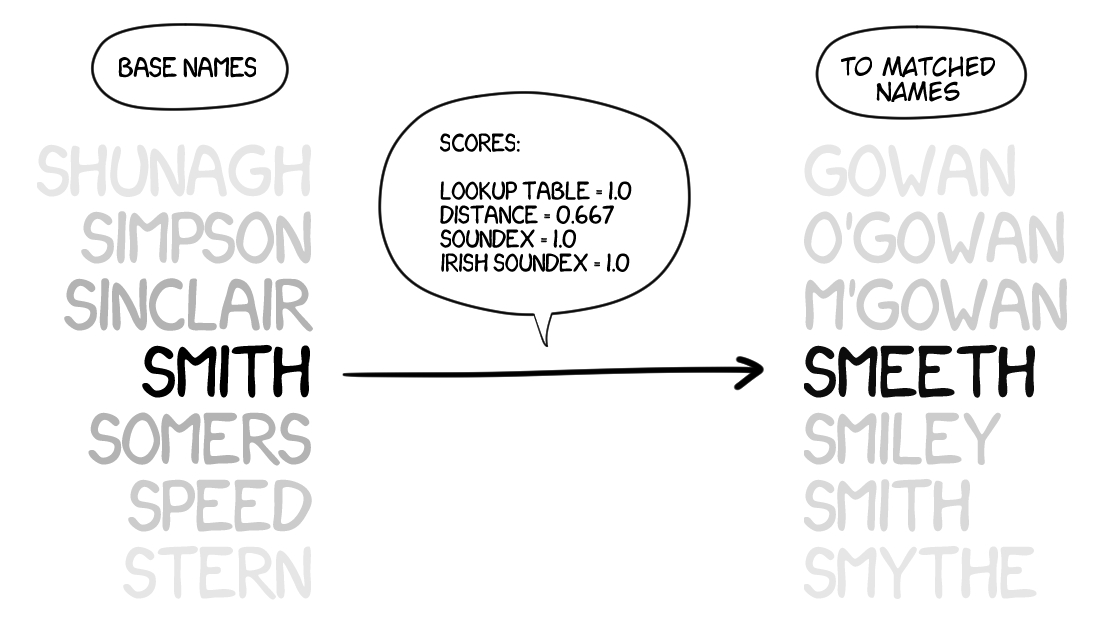
\includegraphics[width=11cm]{gfx/base_tmn}
\caption[\emph{Base name} `SMITH' comparing to \emph{to-match name} `SMEETH'.]{\emph{Base name}
`SMITH' comparing to \emph{to-match name} `SMEETH'. \\
Scores of each matching algorithms
are presented in the bubble above the arrow.}
\label{fig:base_tmn}
\end{figure}

Figure \ref{fig:base_tmn} shows a snapshot of an attempt to match between
\emph{base name} `SMITH' against \emph{to-match name} `SMEETH'.
\emph{Similarity score} for each matching algorithms have been calculated.
And by these scores, we can calculate \emph{overall score} for `SMITH'
and `SMEETH'.

So the next step is to match current \emph{base name}, `SMITH',
against next \emph{to-match name}, `SMILEY'.

Once \emph{base name} `SMITH' completes all \emph{to-match name}\textquotesingle s in their list,
the system then process to the next \emph{base name}, `SOMERS', and start over
the matching process against the whole \emph{to-match name} list again, from
start to the end.

\section{Weighting matching algorithms}

We realised that, for matching names, each matching algorithms
should not be treated as all the same priority. For example, for Irish names,
it would be better if we favour \emph{Irish soundex} over the
traditional \emph{Soundex}, because it produces more accurate result.

By this idea we also implement \emph{weight} for each matching algorithm.
We will suggest initial values, but also allow client to change these values.
Table \ref{table:weights} states these suggested initial weights.

\begin{table}[H]
  \myfloatalign
  \setlength{\tabcolsep}{0.3cm}
  \begin{tabular}{c c}
    \toprule
    \tableheadline{Matching algorithm} & \tableheadline{Weight} \\
    \midrule
    Levenshtein distance & 1 \\
    Soundex & 3 \\
    Irish soundex & 6 \\
    Lookup table & 10 \\
    \bottomrule
  \end{tabular}
  \caption{Matching algorithm weights.}
  \label{table:weights}
\end{table}

By summarise products of each matching algorithm \emph{similarity score}
and its weight, dividing by sum of all weight, we can obtain
\emph{overall weighted score} (OWS). This sentence can be represented
by equation \ref{eq:ows}.

\begin{equation}
  \begin{gathered}
    OWS = \frac{
      \displaystyle\sum_{i=1}^{n} (s_i \times w_i)
    }{
      \displaystyle\sum_{i=1}^{n} w_i
    }
  \end{gathered}
  \label{eq:ows}
\end{equation}

Where $s$ and $w$ are \emph{similarity score} and weight of
matching algorithm $i$ respectively. $n$ is number of available
matching algorithms.

This \emph{overall weighted score} will represent
each matching and all results will be sorted by this score.
Usage and calculation of this weighting will be described in more detail
in the next section (\ref{sec:actualsys}).

\section{Actual system}
\label{sec:actualsys}

Following our basic idea from previous sections, we then design the
architecture of our system.

Suppose we have two inputs, list of \emph{base names} of length $b$,
and list of \emph{to-match names} of length $t$. We need to
process the matching for $b \times t$ times. We call this single
matching between \emph{base name} and \emph{to-match name}
as \emph{matching cycle}.

In this following figure \ref{fig:overall} we once again show a snapshot
of an attempt to match between \emph{base name} `SMITH'
against \emph{to-match name} `SMEETH'. But now in a \emph{matching cycle} style.

\begin{figure}[H]
\centering
\captionsetup{justification=centering}
\makebox[\textwidth][c]{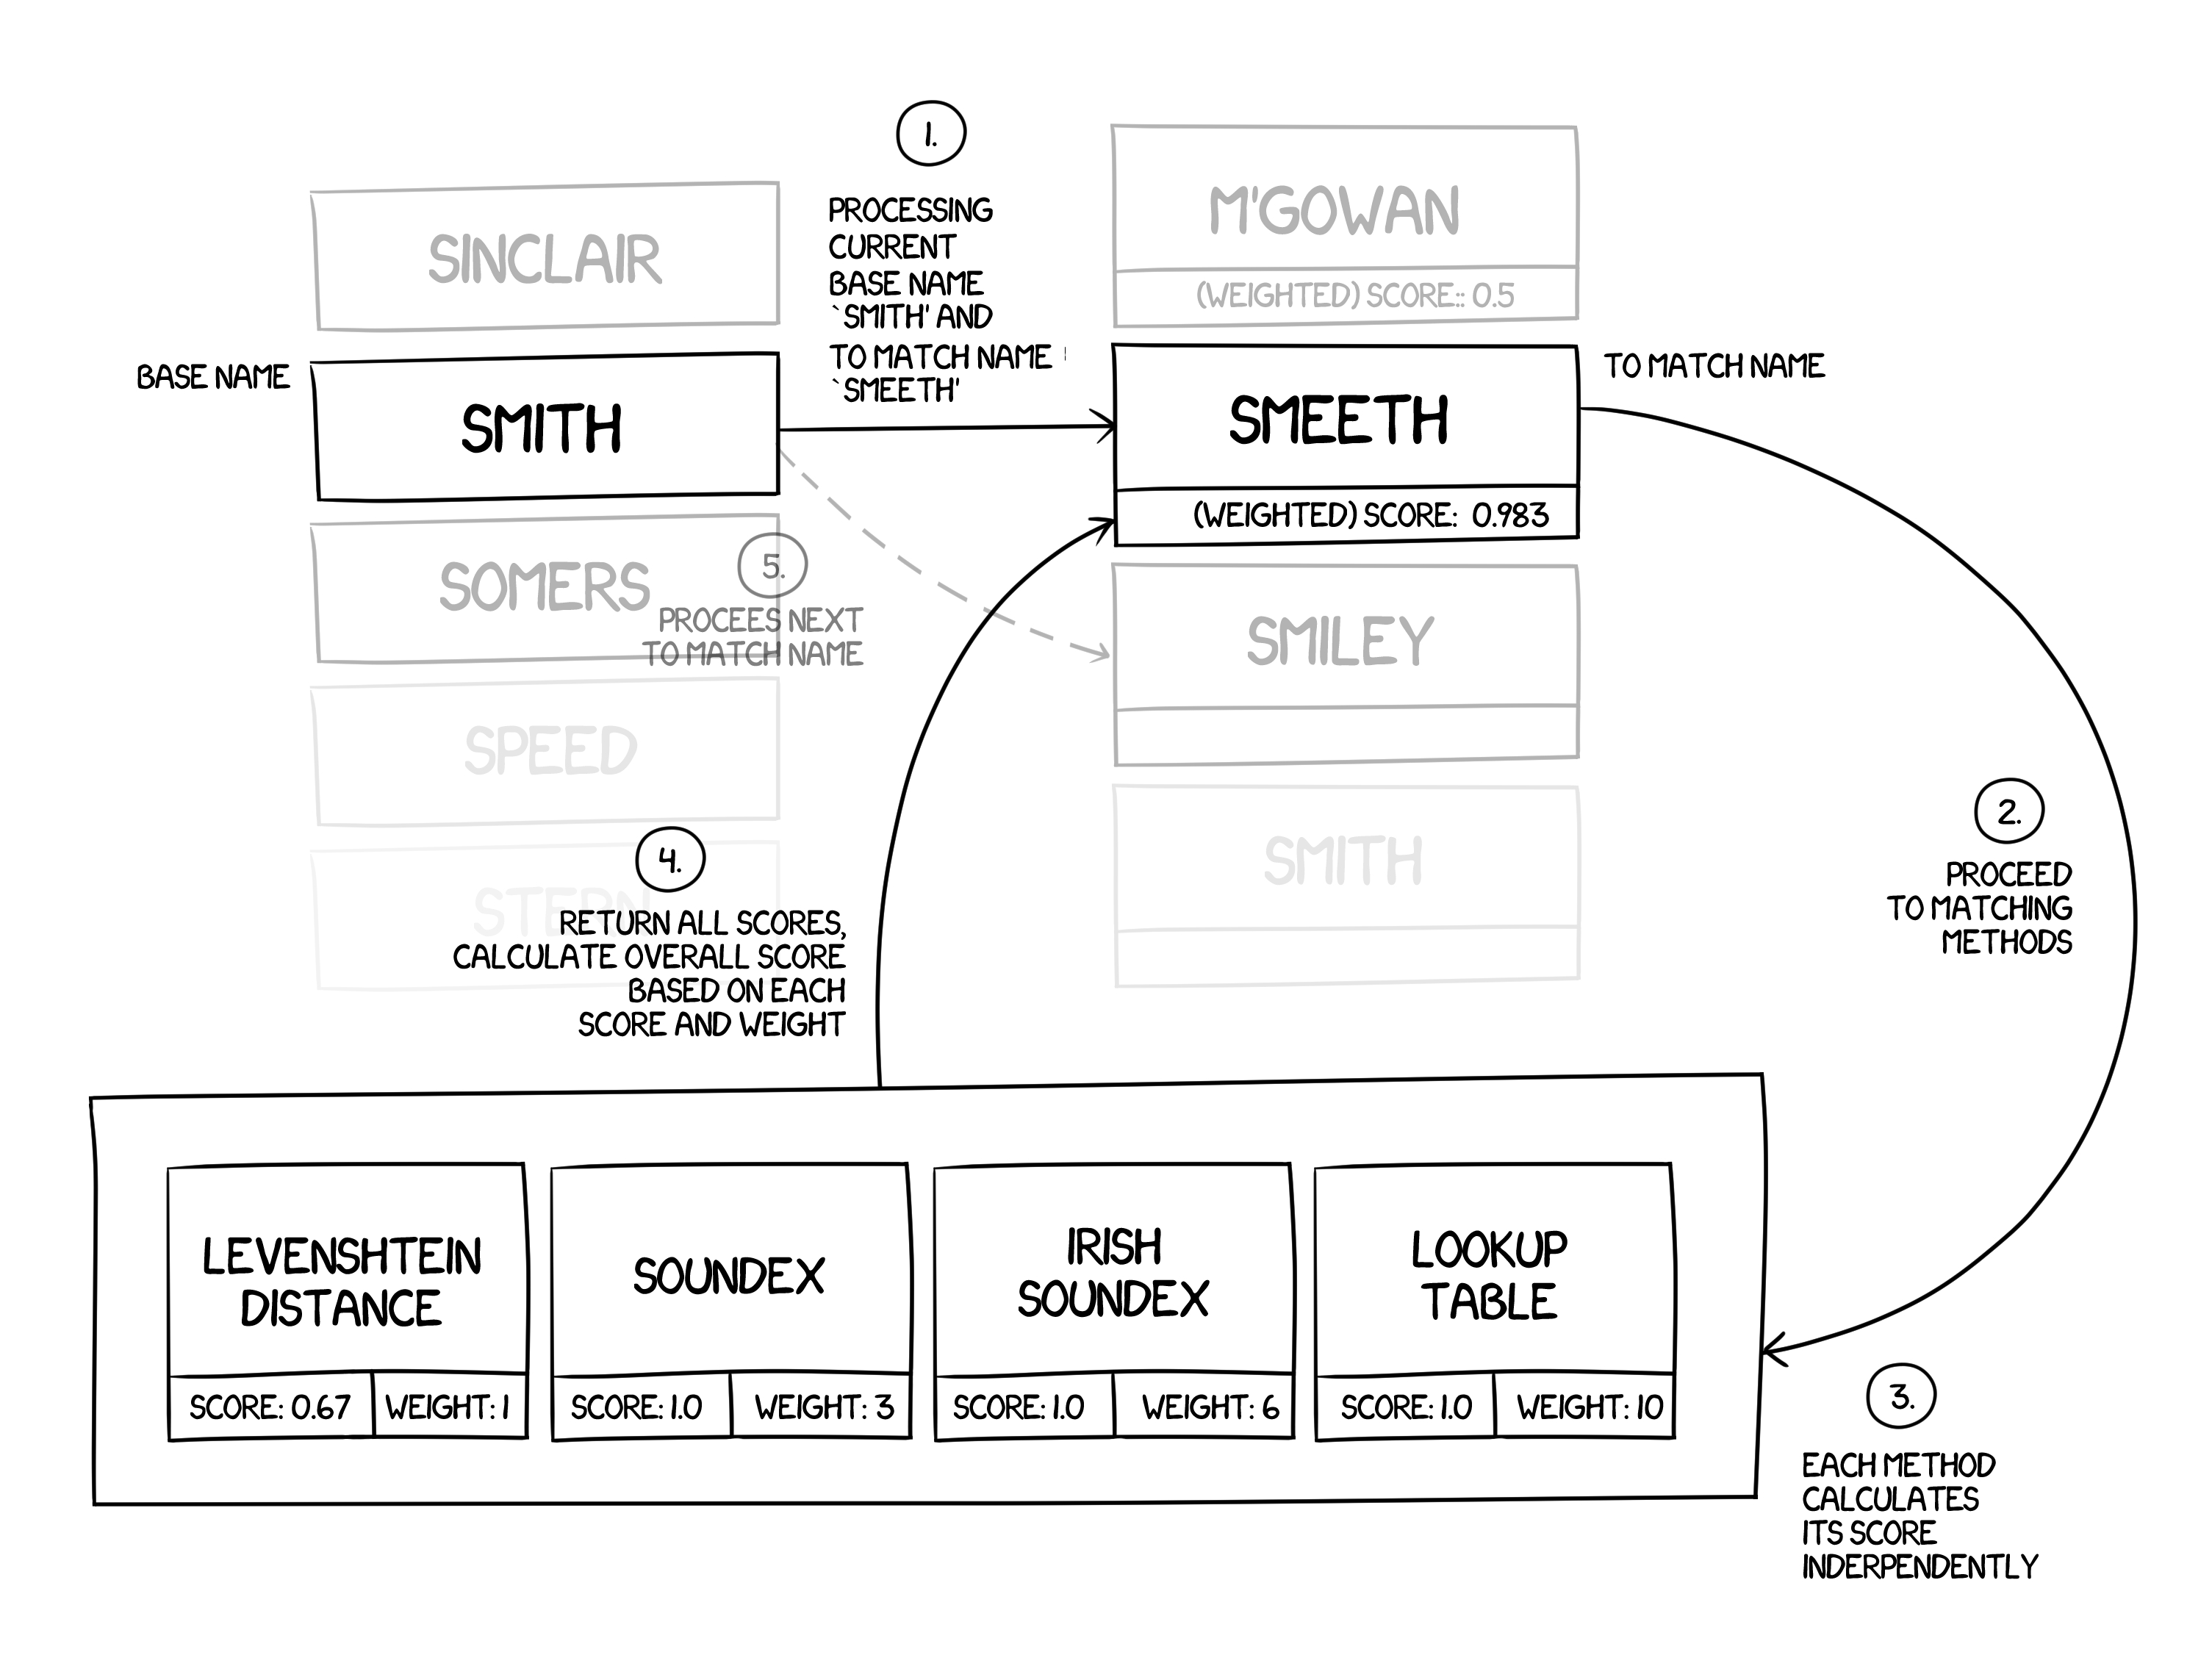
\includegraphics[width=16cm]{gfx/overall}}
\caption{One matching cycle.}
\label{fig:overall}
\end{figure}

One matching cycle consists of 5 steps as shown in figure \ref{fig:overall}.

\begin{enumerate}
  \item Processing current \emph{base name} `SMITH' and \emph{to-match name} `SMEETH'
  \item Proceed to matching algorithms.
  \item Each algorithm calculates its score indepedently.
    \begin{enumerate}
      \item Levenshtein distance between `SMITH' and `SMEETH' is 2
        (1 substitution of \emph{I} to \emph{E} and 1 insertion of \emph{E}).
        So \emph{similarity score} is $(6 - 2) \div 6 = 0.667$ where 6 comes from thelength of the
        longer string, \emph{SMEETH}.

        Weight of this algorithm is 1.

        \textsc{$\therefore$ weighted score = $0.667 \times 1 = 0.667$}
      \item Soundex of both `SMITH' and `SMEETH' are \texttt{S530} so their
        \emph{similarity score} is 1.0.

        Weight of this algorithm is 3.

        \textsc{$\therefore$ weighted score = $1.0 \times 3 = 3.0$}
      \item Irish soundex of both `SMITH' and `SMEETH' are \texttt{S530} so their
        \emph{similarity score} is 1.0.

        Weight of this algorithm is 6.

        \textsc{$\therefore$ weighted score = $1.0 \times 6 = 6.0$}
      \item References between `SMITH' and `SMEETH' is found in the
        Lookup table via group 1897. so their \emph{similarity score} is 1.0

        Weight of this algorithm is 10.

        \textsc{$\therefore$ weighted score = $1.0 \times 10 = 10.0$}
    \end{enumerate}
  \item Return all scores and then calculate \emph{overall weighted score}
    for `SMITH' and `SMEETH'. Sum of the scores is
    $0.667 + 3.0 + 6.0 + 10.0 = 19.667$. Sum of the weights is
    $1 + 3 + 6 + 10 = 20$. Therefore the \emph{overall weighted score} is
    $19.667 \div 20 = 0.983$.
  \item Matching cycle for `SMITH' and `SMEETH' is finished with
    \emph{overall weighted score} 0.983.
    Now the system will proceed to the next \emph{to-match name} `SMILEY'.
    Matching cycles for \emph{base name} `SMITH' will continue until
    the end of \emph{to-match name} list. After that it will start
    matching cycles for \emph{base name} `SOMERS' from the start of
    \emph{to-match names}, and so on.
\end{enumerate}

Once all cycles are fully finished for every \emph{base names} and
\emph{to-match names}, we will get all \emph{overall weighted scores}
ready. So we can sort and present in web interface (section \ref{sec:wi}), or return
as a result in web service (section \ref{sec:ws}).

\section{MVC}
\label{sec:mcv}

\section{Web Interface}
\label{sec:wi}

\section{Web Service}
\label{sec:ws}
